\documentclass[a4paper,11pt]{scrartcl}

\usepackage[ngerman]{babel} 
\usepackage[T1]{fontenc}
\usepackage[utf8]{inputenc}
\usepackage{hyperref}

\usepackage{amsmath,amsfonts,amssymb}
\usepackage{graphicx}
\usepackage{siunitx}

\usepackage{epstopdf}

\setcounter{section}{2}


\begin{document}
\hfill Alexander Schnapp

\hfill Max Menges

\begin{center}
\underline{\Huge{Intro HPC: Blatt 2}}\\
\large{04.11.1014}\\
\end{center}

\subsection{MPI Ring Communication}

Der Quelltext zur aufgabe liegt unter \verb+../2/2_1/2_1.cpp+. In dem Ordner liegt auch ein \verb+Makefile+ zum Compilieren und Ausfürhren. Benutzung: 

\begin{table}[!ht]
    \begin{tabular}{ll}
    \verb+make+& Compile \\ 
    \verb+make clean+& Bin und \verb+*.o+ löschen  \\ 
    \verb+make run proc=$p msg=$m v=$v +& Ausfrühren mit \verb+$p+ Prozessen, \verb+$m+ Nachrichten \\
    \verb+make run_opt proc=$p msg=$m v=$v+&  Siehe \verb+run+, aber mit optimiertem Mapping\\ 
    \end{tabular}
\end{table}

Parameter \verb+$v+ für Ausgabe der Zeit, \verb+1+ für nett formatiert, \verb+0+ nur gesamte Zeit und pro Nachricht.\\

Plot unten zeigt durchschnittliche Zeit pro Nachricht bei 12 Prozessen. Jeder run wurde 20 mal gemessen um den Fehler in der Laufzeit zu bestimmen (stabilste message size $m$). Obwohl 5 Nachrichten eine kleine Abweichung haben, haben wir für die Messung 10 Nachrichten genommen um ein wenig bessere Statistik machen zu können.

\begin{figure}[!ht]
    \centering
    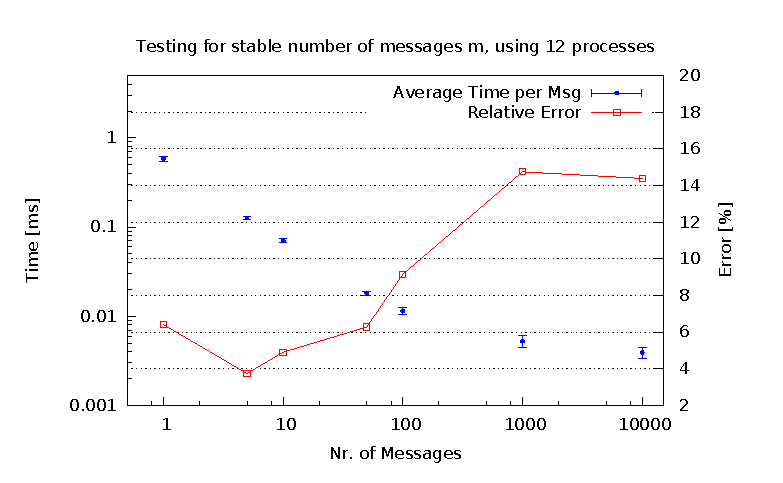
\includegraphics[width=0.7\textwidth,keepaspectratio]{2_1/data/runs.eps}
\end{figure}

Messung der Ausführungsdauer bei 24 Prozessen, 10 Nachrichten pro Prozess und Mapping \verb+creek01,..,creek08+. Das Programm wurde auch wieder für jede Prozessanzahl 20 mal ausgeführt. Die Ergebnisse sind unten geplottet. Die Zeit pro Nachricht steigt mit der Anzahl Prozesse leicht an und liegt bei $\approx$ \SI{0.07}{\milli\second}.\\


\begin{figure}[!ht]
    \centering
    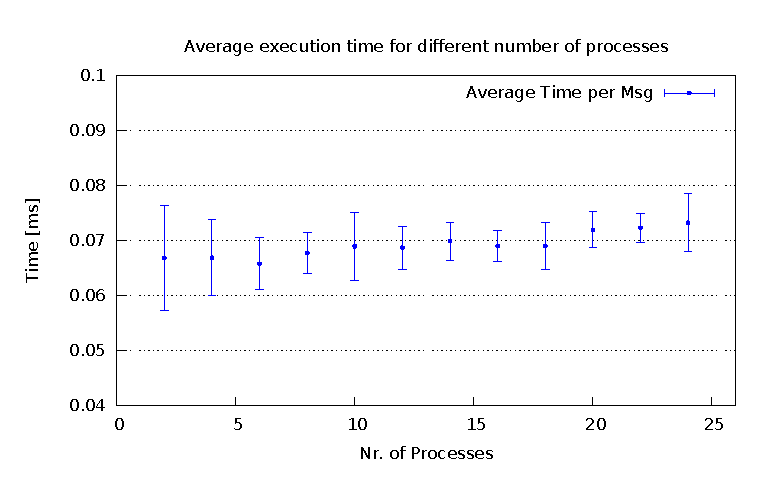
\includegraphics[width=0.7\textwidth,keepaspectratio]{2_1/data/time.eps}
\end{figure}

\sisetup{separate-uncertainty}

Für den letzen Teil der Aufgabe wurde das Mapping für bessere Performance geändert. Jeder Prozess sendet an seinen Nachfolger, da dieser durch das "normale" Mapping jeweils auf einem anderen Rechner liegt, muss jede Nachricht einmal durchs Netzwerk, was Zeit kostet. 
Das Mapping wurde so angepasst, dass die ersten 8 Prozesse (\verb+creek04+ hat laut \verb+nproc+ 8 Cores) auf \verb+creek04+ laufen und die nächsten 4 auf \verb+creek05+. Dadurch sind nur zwei Nachrichten über das Netzwerk nötig, alle anderen laufen nur von Core zu Core in der selben Maschine. \\

Dadurch verringert sich die Zeit pro Nachricht auf \SI[multi-part-units=single]{0.0292(26)}{\milli\second} (siehe Plot). Das optimierte Mapping ist damit $\approx$ $2.35$ fach schneller.

\begin{figure}[!ht]
    \centering
    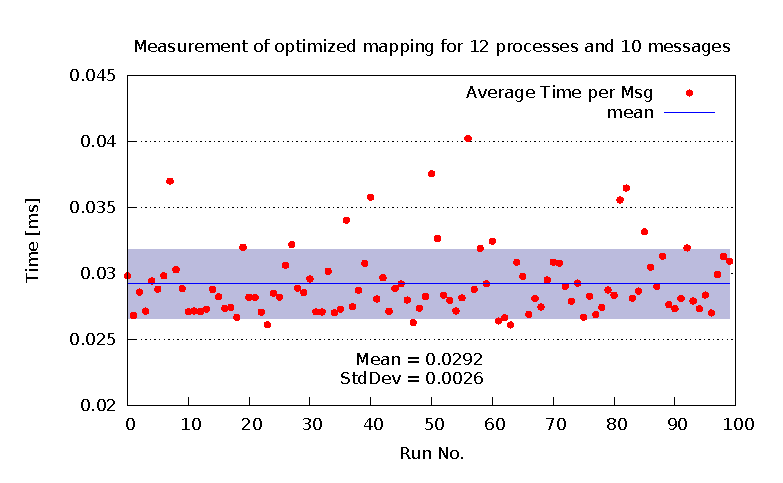
\includegraphics[width=0.7\textwidth,keepaspectratio]{2_1/data/opt.eps}
\end{figure}




\subsection{Barrier Synchronization}


\subsection{Matrix multiply – sequential version}

Der Quelltext zur aufgabe liegt unter \verb+../2/2_3/2_3.cpp+. In dem Ordner liegt auch ein \verb+Makefile+ zum Compilieren und Ausfürhren. Benutzung: 

\begin{table}[!ht]
    \begin{tabular}{ll}
    \verb+make+& Compile \\ 
    \verb+make run n=$n runs=$x opt=$opt+ & Matrix Multiplation mit $\$n*\$n$-Matritzen, \verb+$x+ mal ausgeführt. \\
    \end{tabular}
\end{table}
Parameter \verb+$opt+ wählt zwischen naiver und optimierter Implementierung.\\

Ausgeführt auf \verb+creek04+ braucht die nicht optimierte Matrix Multiplikation im Schnitt \SI{333.19}{\second}. Die Matrix Multiplikation besteht aus 3 ineinander verschachtelten Schleifen und bei jedem Durchlauf der inneren Schleife werden zwei floating point Operationen (1 \verb+add+, 1 \verb+mul+) ausgeführt, insgesamt also $2\cdot n^3$ floating point Operationen pro Matrix Multiplikation. Bei $n=2048$ ergibt dies $\approx 0.05155 GFLOPS$. 

\begin{figure}[!ht]
    \centering
    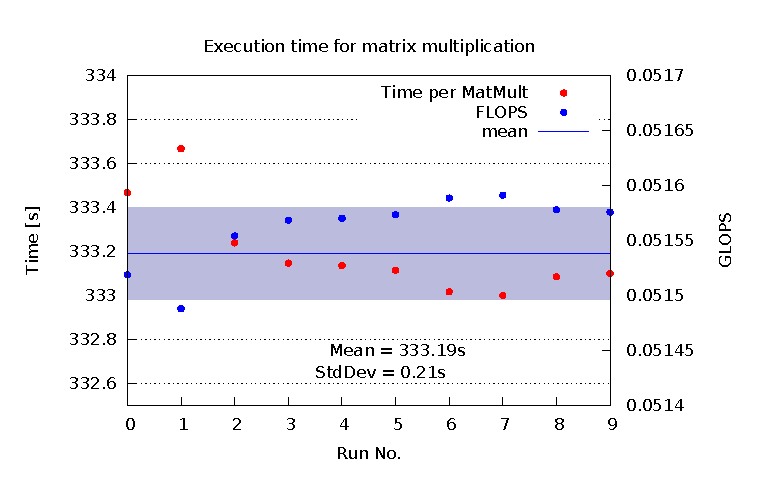
\includegraphics[width=0.7\textwidth,keepaspectratio]{2_3/data/matmult.eps}
\end{figure}

Intel gibt für den \emph{Xeon E5-1620}\footnote{\url{http://download.intel.com/support/processors/xeon/sb/xeon_E5-1600.pdf}} theoretische $115.2$ GFLOPS bei 4 Cores an. Mit einem Core sollten somit noch immer noch $28.8$ GFLOPS zu erreichen sein.

Der performance gap kommt von der größe der Matrix und der Zugriffszeit auf den Hauptspeicher bei einem Cache Miss. Da die Matrix nicht mehr komplett in den Cache passt (32 MB bei $n=2048$ double-precision), muss ständig auf den Hauptspeicher zugegriffen werden. Da außerdem die $\mathbf{B}$ Matrix (bei $\mathbf{C}=\mathbf{A}\times \mathbf{B}$) zeilenweise durchlaufen wird, werden -- je nach Matrix und Cache-Line größe -- nur ein oder wenige Einträge pro Cache-Line verwendet. \\


\begin{figure}[!ht]
    \centering
    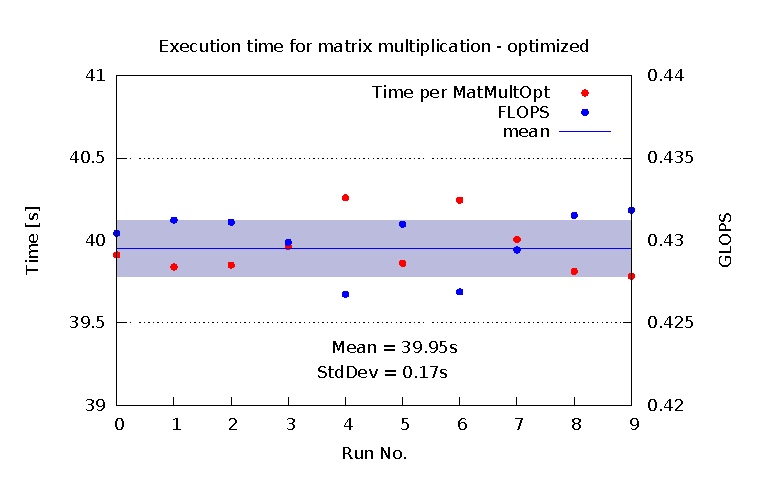
\includegraphics[width=0.7\textwidth,keepaspectratio]{2_3/data/opt.eps}
\end{figure}

Um die performance zu verbessern kann man nun die Reihenfolge der \verb+j+ und \verb+k+ Schleifen vertauschen. Dies sorgt dafür, dass nun sowohl in $\mathbf{A}$ als auch in $\mathbf{B}$ jeweils auf zusammenhängenden Speicher zugegriffen wird, was weniger cache misses zur folge hat, da jetzt jeder Matrixeintrag in der Cache-Line verwendet wird.

Damit verbessert sich die Performance um einen Faktor $\approx 8.34$ gegegnüber der naiven Implementierung. Die benötigte Zeit wird auf \SI{39.95}{\second} reduziert und die GFLOPS auf $0.43$ erhöht. 

Alternativ könnte man auch die Schleifen unverändert lassen und den Zugriff auf $\mathbf{B}$ von \verb|b[k*size+j]| zu \verb|b[j*size+k]| ändern. Das sorgt auch dafür, dass jeweils auf zusammenhängenden Speicher zugegriffen wird. Außerdem ändert sich die Indizierung von $\mathbf{C}$ nicht so häufig, dadurch entfallen einige Speicherzugriffe.
Die Performance kann weiter auf $0.47 GFLOPS$ erhöht werden. Allerdings entspricht dies jetzt der Multiplikation mit der transponierten von $\mathbf{B}$: $\mathbf{C}=\mathbf{A}\times \mathbf{B}^\intercal$

\begin{verbatim}
void mat_mult_opt(double* a, double* b, double* c,int size){
    for (int i = 0; i < size; i++){
        for (int k = 0; k < size; k++){
            for (int j = 0; j < size; j++){
                c[i*size+j] += a[i*size+k] * b[k*size+j];
            }
        }
    }
}

void mat_mult_trans(double* a, double* b, double* c,int size){
    for (int i = 0; i < size; i++){
        for (int j = 0; j < size; j++){
            for (int k = 0; k < size; k++){
                c[i*size+j] += a[i*size+k] * b[j*size+k];
            }
        }
    }
}
\end{verbatim}


\end{document}
